\section{{[}TEMPLATE EVENTO STORICO{]}}\label{template-evento-storico}

\section{{[}Evento Storico{]}}\label{evento-storico}

\begin{center}\rule{0.5\linewidth}{0.5pt}\end{center}

\begin{figure}
\centering
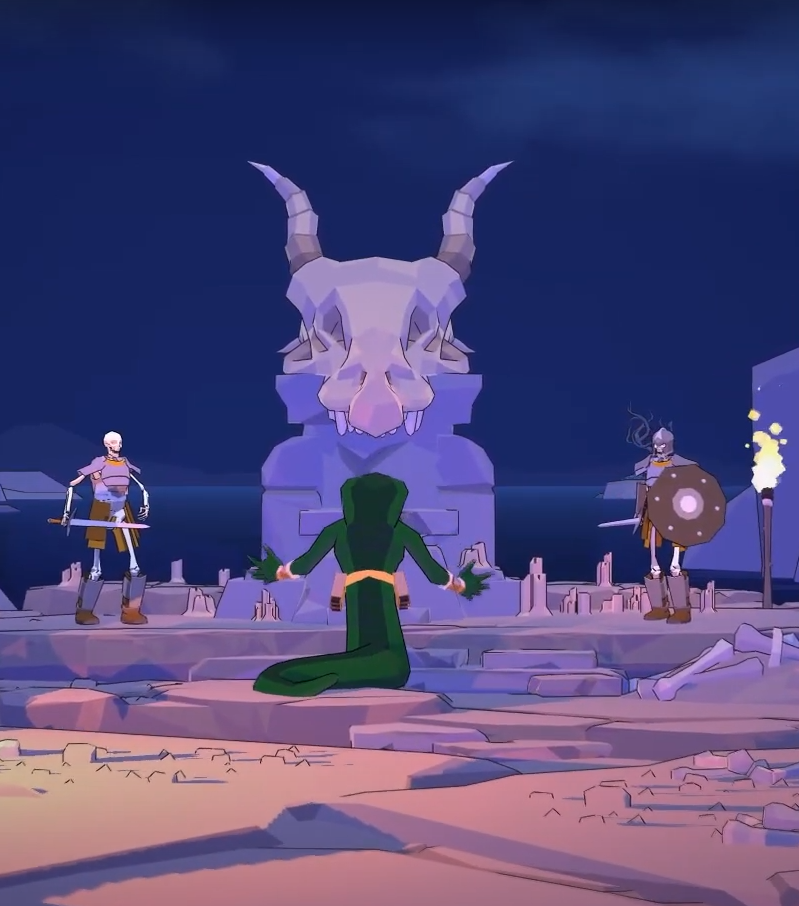
\includegraphics{chrome_LPW012t3FZ.png}
\caption{chrome\_LPW012t3FZ.png}
\end{figure}

Informazioni Generali

Tipo:

Data:

Durata:

Luogo:

Partecipanti:

Risultati:

\begin{center}\rule{0.5\linewidth}{0.5pt}\end{center}

\begin{center}\rule{0.5\linewidth}{0.5pt}\end{center}

\subsection{1. Descrizione Generale}\label{descrizione-generale}

\begin{center}\rule{0.5\linewidth}{0.5pt}\end{center}

\begin{figure}
\centering
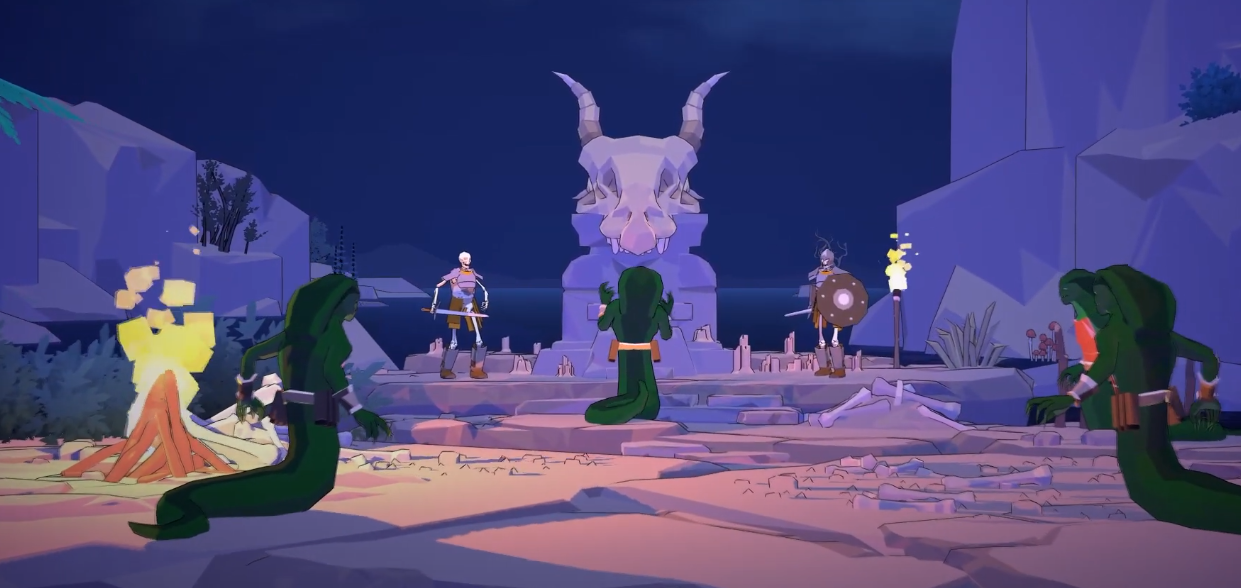
\includegraphics{chrome_YShQkc70No.png}
\caption{chrome\_YShQkc70No.png}
\end{figure}

{[}Historical event{]} was a {[}type of event{]} that involved
{[}organization{]}, lead by {[}character{]}.

\begin{quote}
Quote about {[}historical event{]}
\end{quote}

\subsection{2. Background Storico}\label{background-storico}

\begin{center}\rule{0.5\linewidth}{0.5pt}\end{center}

{[}Historical event{]} was a {[}type of event{]} that occurred in
{[}location{]} around {[}time{]}. A {[}type of organization{]} called
{[}name of organization{]} embarked on a campaign supported by {[}larger
organization{]}. Their goal was to {[}objective{]}. This culminated in
{[}preceding event{]} leading to {[}this event{]}.

\subsection{3. Aftermath \& Conseguenze a Lungo
Termine}\label{aftermath-conseguenze-a-lungo-termine}

\begin{center}\rule{0.5\linewidth}{0.5pt}\end{center}

\subsection{4. {[}Evento Storico{]} Nel Mito e nel
Folklore}\label{evento-storico-nel-mito-e-nel-folklore}

\begin{center}\rule{0.5\linewidth}{0.5pt}\end{center}

\subsection{5. Player Predispositions /
Archetypes:}\label{player-predispositions-archetypes}

\begin{center}\rule{0.5\linewidth}{0.5pt}\end{center}

{[}Event{]} will definitely remind player of {[}thing player is familiar
with---e.g.~American Civil War, Bubonic Plague, the Mongol invasion{]}
